%!TEX root = ../course_work.tex

\section{Методы}
\subsection{Методы сегментации и классификации}

\subsubsection*{NormResSE-UNet3+}
В работе \cite{NormRes} решается задача сегментации опухолей головы и шеи с помо-
щью сверточной нейронной сети, а также задача предсказания выживаемости
пациентов с помощью регресионной модели. \par 
Авторы предлагают производить сегментацию опухолей головы и шеи
по ПЭТ/КТ изображениям, используя полномасшатбную сеть архитектуры
3D UNet3++ \cite{Unet} с механизмом, имитирующим когнитивное внимание. Предложенная модель, NormResSE-UNet3+ была обучена с ги-
бридной функцией потерь, состоящей из Log Cosh Dice и Focal loss. Далее,
предсказанные карты сегментации дополнительно уточняются с помощью ме-
ханизма постпроцессинга - Conditional Random Fields, чтобы уменьшить чис-
ло ложноположительных ответов и улучшить сегментацию границы опухоли.
Для решения задачи предсказания выживаемости предлагается регресионная
модель CoxPH относительной опасности, использующая комбинацию клинических признаков, а также признаков, полученных
при глубоком обучении на ПЭТ/КТ-изображениях.

Для задачи сегментации была использована трилинейная интерполяция
ПЭТ и КТ-изображений. Интесивность ПЭТ была нормализована с помощью Z-score, а 
интенсивность КТ приведена к [-1,1].
Данные для предсказания выживаемости были обработаны с учетом
пропущенных значений. \par

Архитектура предложенной сети NormResSE-UNet3+: 
\begin{itemize}
    \item На вход подается тензор, размерности 2x144x144x144, состоящий из конкатенации
    ПЭТ и КТ изображений.
    \item Энкодер состоит из residual squeeze-and-excitation блоков, первый блок из которых 
    содержит 24 фильтра. Размерность выхода энкодера - 384x3x3x3
    \item Путь декодирования состоит из полномасштабных соединений и модуля, содержащего 
    правильную разметку изорбражений (ground truth).
    \item У декодера одноканальный выход размерности 1х144х144х144
\end{itemize}

\begin{minipage}{1.0\linewidth}
    \centering
    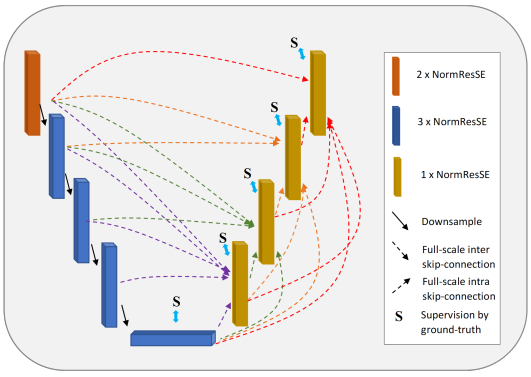
\includegraphics[scale=0.5]{ann6_arch.png}
\end{minipage}
\\

Было обучено несколько моделей нейронных сетей для задачи сег-
ментации опухолей головы и шеи. Предложенная регрессионная
модель CoxPH, а также модель NormResSE-UNet3+ показали лучший результат по сравнению с другими предшемтвующими моделями.


\begin{minipage}{1.0\linewidth}
    \begin{center}
    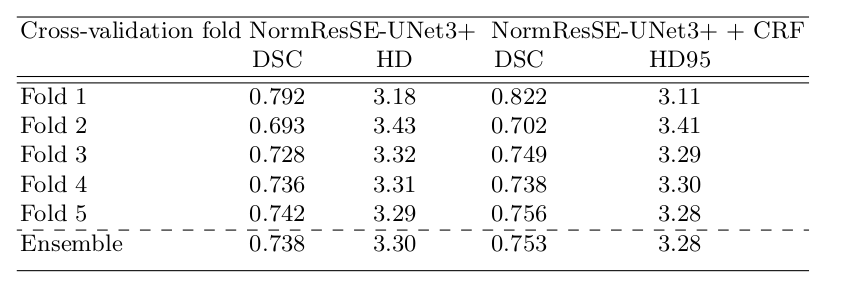
\includegraphics[scale=0.5]{ann6_res.png}\\
   % \caption{\scriptsize{Количественные результаты сегментации}}
\end{center}
\end{minipage}
\\


\subsubsection*{Cascaded Unet}
Точная сегментация и реконструкция медицинских 3D изображений
способны дать больше необходимой информации о прогрессировании забо-
левания и позволяют терапевту спланировать успешный курс лечения для
больного. В данной работе \cite{Cascaded} авторы представляют каскадный вариант попу-
лярной сети UNet \cite{Unet}, который итеративно улучшает результаты сегментации,
полученные на предыдущих шагах.\par
Предложенный метод может быть представлен как цепь классификаторов 
\(C_i\), одинаковой топологии F, у каждого из которых свой собственный 
набор параметров \(W_i\) для оптимизации в течение обучения.
Результат вычисления \(i\)-го шага представляется следующим образом: 
\(Y_i=F(X_i,Y_{i-1}, Y_{i-2}, W_i)\). Каждый из базовых блоков \(C_i\) - это
сеть архитектуры UNet, измененная для задачи сегментации глиом. В сравнении 
со стандартной архитектурой UNet, в предложенной модели используется несколько 
энкодеров, которые раздельно обрабатывают входные данные. Также, предложен метод объединения 
их выхода: в UNet \(i\)-й выход декодера зависит от выхода соответствующего 
энкодера и выхода предыдущего декодера - \(d_i^{t}=f(e_i^{t}, d^{t}_{i-1})\). 
Раскрывая первую свертку \(f\), получаем - \(d_i^{t}=g(W_{i,e}^{t}e_i^{t}+W_{i},d^{t}d^{t}_{i-1})\).
Далее предлагается объединить контекст, полученный на более низких слоях, 
добавляя соответствующий выход \(y^t\), поэтому \(d_i^{t}=g(W_{i,e}^{t}e_i^{t}+W_{i,d}^{t}d^{t}_{i-1}+W_{i,y}^{t}y^{t-i})\).
\par 

\begin{minipage}{1.0\linewidth}
    \begin{center}
        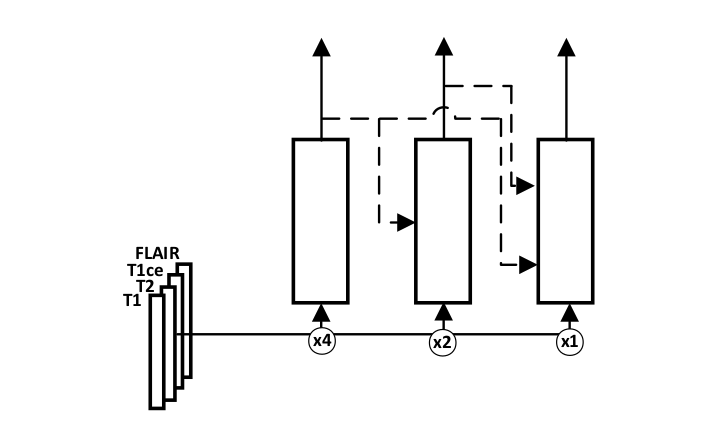
\includegraphics[scale=0.6]{ann7_arch.png} \\
        % \caption{\scriptsize{Схематическое представление метода, описанного в статье.
        % T1, T2, T1ce, FLAIR - входные модальности МРТ-изображения, x4,x2 - понижающий
        % фактор входа сети. Пунткирные линии - соединения между блоками \(C_i\).}}
    \end{center}
\end{minipage}


В качестве датсета использовался набор МРТ-изображений BraTS2018 \cite{BraTS}. Результат сегментации  оценивался по метрике Dice, отдельно вычисленной
для следующих частей опухоли: WT (whole tumor) -  вся опухоль, ET (enchancing tumor) - 
усиливающаяся часть опухоли и TC (tumor core) - ядро опухоли. Предложенный алгоритм автоматической сегментации опухолей головного мозга по МРТ-зображениям, который решает также
проблему мультимодального входа и показывает хорошие резльтаты по сравнению с моделью UNet.

\subsubsection*{Medical Transformer}

Сверточные нейронные сети сравнительно плохо понимают зависимости между признаками, которые находятся на дальнем расстоянии друг от друга
в изображениях. Недавно предложенные архитекутры сетей, основанные на
трансформерах \cite{Transformers}, используют механизм самовнимания \cite{SelfAttention} для шифрования дальних
зависимостей и выявляют наиболее заметные представления. Эти наблюдения
мотивировали авторов статьи исследовать решения, в основе которых лежат
трансформеры и изучить возможность использования архитектур нейронных
сетей с трансформерами в задачах медицинской сегментации. \cite{MedT} \par 
В данной работе предлагается закрытый, чувствительный к расположению axial 
attention механизм, который хорошо показывает себя на малых
наборах данных. Также, вводится эффективная методология обучения Local-
Global (LoGo) для трансформеров и Medical-Transformer (MedT) - метод,
построенный на основе двух вышеперечисленных предложенных концепций,
разработанный специально для сегментации медицинских изображений, который успешно улучшает производительность по сравнению со сверточными
нейронными сетями и сетями чисто attention архитектуры на трех разных датасетах. Предложенные методы
превосходят существующие в задаче сегментации медицинских изображений
не требуя при этом большого набора тренировочных данных.\\


\begin{minipage}{1.0\linewidth}
    \begin{center}
        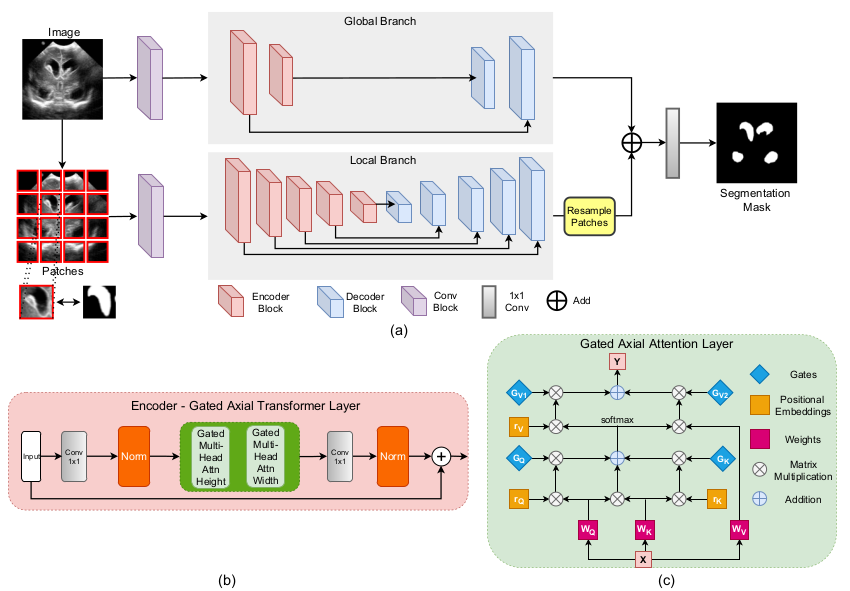
\includegraphics[scale=0.45]{ann18_arch.png} 
        % \caption{\scriptsize{
        %    Архитектура MedT.
        % }}
    \end{center} 

\end{minipage} 

Local-Global training:\\

Чтобы улучшить общее понимание изображения, предлагается использовать 
два ответвления сети - глобальная ветвь, которая работает с 
изображением оригинальной размерности и локальная ветвь для работы с патчами. 
В локальной ветви создается 16 патчей размера \(I/4 \times I/4\), каждый патч 
пропускается через сеть и выходные карты признаков resampled, основываясь на их расположении, 
чтобы получить итоговые карты признаков. К итоговым картам двух ветвей применяется 
свертка \(1\times 1\) и на выходе получается маска сегментации. 
Такая стратегия улучшает производительность, так как глобальная ветвь 
фокусируется на высокоуровневой информации, а локальная лучше определяет детали.\\



\subsubsection*{AFTer-UNet}

Последние достижения в моделях, основанных на трансформерах \cite{Transformers} 
притянули внимание исследователей для изучения данных техник в сегментации медицинских изображений. Особенно часто 
трансформеры используются совместно с U-Net подобными моделями (и их производными), которые
показали хороший результат в обработке двумерных и трехмерных изображений. В существующих методах, основанных на двумерных изображениях,
сверточные слои напрямую заменяются трансформерами, либо трасформер
применяется в качестве дополнительного промежуточного энкодера между
энкодером и декодером U-Net. Однако, при таком подходе пространственная
информация используется не полностью, сеть видит только срезы трехмерного изображения,
 не учитывая связи в целом трехмерном изображении. \par

 Для того, чтобы трансформер мог находить связи между признаками, 
 находящимися на далеком расстоянии в трехмерных медицинских изображениях,
 в данной работе\cite{ATerUnet} предлагается архитектура Axial Fusion Transformer UNet (AFTer-UNet).
 AFTer-UNet следует архитектуре U-Net \cite{Unet}, которая состоит из двумерного сверточного энкодера 
 и декодера, но между ними авторы разместили промежуточный axial fusion transformer энкодер, 
 для того, чтобы связать контекстную информацию из соседних срезов. Промежуточный 
 энкодер снижает вычислительную сложность тем, что сначала отдельно вычисляется 
 фокус (attention) вдоль осей и внутри одного среза, а потом полученная ифнормация 
 объединяется для составления финальной карты сегментации. \par
 
 \subsubsection*{Vit-V-Net}

В данной работе \cite{VitVNet} исследуется применение ViT \cite{Transformers} в объемных медицинских изображениях. 
Авторы предлагают ViT-V-Net \cite{VNet}, которая воплощает в себе гибридную архитектуру
„сверточная нейронная сеть-трансформер“ (ConvNet-Transformer) для приме-
нения self-supervised метода в исследовании трехмерных медицинских изоб-
ражений.\par 

В предложенном методе ViT была применена к высокоуровневым признакам изображений, 
что требовало от сети выявить зависимости между
точками, находящимися на дальнем расстоянии. Наивное применение ViT
к полномасштабным изображениям приводит к увеличению вычислительной
сложности. Поэтому, изображения сначала были закодированы с помощью
нескольких сверточных слоев и слоев max-pooling для получения объектов,
содержащих высокоуровневые признаки. Далее, в ViT, высокоуровневые признаки 
делятся на патчи, а затем патчи отображаются в скрытое пространство
с помощью обучаемой линейной проекции (например, patch embedding). Затем, 
результирующие патчи подаются в энкодер трансформера, а полученный
выход декодируется V-Net подобным декодером.

\subsubsection*{CaraNet}

Только малая часть 
 исследований учитывает размер интересующих объектов на изображении
 и поэтому многие модели показывают плохой результат при сегментации
 объектов малого размера, что сильно влияет на диагностику заболевания.
 В данной работе \cite{CaraNet} предлагается нейросетевая модель Context Axial
 Reserve Attention Network (CaraNet), которая способна улучшить 
 результаты сегментации малых объектов по сравнению с уже существующими
 моделями. \par

 В архитектуре CaraNet используется параллельный частичный декодер 
(parallel partial decoder) для генерации высокоуровневой семантической
карты и набор операций (Context and Axial Reverse Attention) для 
идентификации глобальных и локальных признаков. 
\\Модули CaraNet:
\begin{itemize}
    \item \textit{Parallel partial decoder.} Эксперименты показали,
    что низкоуровненвые признаки вычислительно более сложны и вносят 
    меньший вклад в улучшение результатов сегментации. Поэтому, авторы 
    используют параллельный частичный декодер \(p_d(\cdot)\) для извлечения 
    высокоуровневых признаков \(PD=p_d(f_3,f_4,f_5)\) и получения глобальной карты 
    \(S_g\) из частичного декодера.
    \item \textit{Context module.} Чтобы получить контекстную информацию из высокоуровневых
    признаков, применяется модуль CFP (Channel-wise Feature Pyramid) cо степенью растяжения 
    (dilation rate) \(d=8\). После контекстного модуля можно получить многомасштабные 
    высокоуровневые признаки \(\{f_{3}^{'}, f_{4}^{'}, f_{5}^{'}\}\).
    \item \textit{Axial reverse attention.} Данный модуль состоит из двух частей:
    маршрут по оси (axial attention route) и обратный маршрут (reverse attention route). Глобальная 
    карта \(S_g\) может поймать только приблизительное расположение тканей без структурных деталей, 
    поэтому структурированный регион тканей постепенно добывается стиранием переднего плана 
    объекта с помощью операции reverse attention: \(R_{i}=1-Sigmoid(S_{i})\). По другому 
    маршруту применяется axial attention. Здесь сеть может извлечь глобальные зависимости и 
    локальное представление совершая вычисления по горизонтальной и вертикальной оси. 
\end{itemize}

По сегментации полипов на основе пяти датасетов, предложенная модель CaraNet не 
только превосходит сравниваемые модели по общей производительности, но и на примерах с 
полипами малых размеров. Для дальнейшей оценки эффективности 
сегментации малых объектов с помощью CaraNet был проведен еще 
один эксперимент, уже с участием опухолей ГМ из датасета BraTS 2018 \cite{BraTS}. 
CaraNet была сравнена с PraNet \cite{PraNet} и показала
лучший результат особенно в случаях с очень малыми объектами.

\subsubsection*{3D Self-Supervised Methods for Medical Imaging}

В данной работе \cite{3DSelfSuper} предлагаются трехмерные варианты self-supervised 
методов, которые облегчают обучение нейронной сети на признаках 
по немаркированным трехмерным изображениям, что приводит к снижению
затрат на экспертную аннотацию. Рассмотрены 5 алгоритмов и проведен 
сравнительный анализ на трехмернвх медицинских изображениях (МРТ, КТ).
Выбор алгоритмов обусловен их успешным применением в двумерном случае и тем,
что ни один из них не был расширен до трехмерного на момент выхода статьи.

\par 
Авторы предлагают 5 алгоритмов, которые целиком используют пространственную информацию
3D-изображения. В каждом методе используется энкодер \(g_{enc}\), который 
может быть дообучен под различные задачи.
\begin{itemize}
    \item \textbf{3D Contrastive Predictive Coding (3D-CPC)} \\
    Следуя идее, предложенной в двумерном случае \cite{CPC}, этот метод предсказывает скрытое 
    пространство для следующих (смежных) образцов. Предложенный CPC определяет 
    proxy-задачу, обрезая одинаковые по размеру и перекрывающиеся участки каждого 
    сканирования. Далее, энкодер \(g_{enc}\) сопоставляет каждый входной патч 
    \(x_{i,j,k}\) его скрытому представлению \(z_{i,j,k}= g_{enc}(x_{i,j,k})\). Затем, 
    следующая модель, называемая контекстой сетью \(g_{cxt}\) суммирует скрытые вектора патчей
    контекста \(x_{i,j,k}\) и составляет свой контекстный вектор 
    \(c_{i,j,k}=g_{cxt}(\{z_{u,v,w}\})\), где \(\{z\}\) - это множество скрытых векторов.
    Наконец, так как \(c_{i,j,k}\) захватывает высокоуровневый контент из контекста, который 
    отвечает \(x_{i,j,k}\), это позволяет предсказать скрытые представления следующих(смежных)
    патчей \(z_{i+l,j,k}\), где \(l\geq 0\). Стоит отметить, что в предложенном 3D-CPC
    в качестве \(g_{enc}\) и \(g_{cxt}\) могут использоваться сети любой архитектуры.
    \item \textbf{Relative 3D patch location (3D-RPL)} \\
    В этой задаче пространственный контекст в изображениях используется 
    как богатый источник для семантического представления данных. В предложенной 
    3D версии из каждого входного 3D изображения выбирается сетка из \(N\)
    неперекрывающихся участков \(\{x_{i}\}_{i\in \{1, \cdots N\}}\) случайного расположения. 
    Далее, центральный патч \(x_c\) используется как ссылка, а очередной патч \(x_q\)
    выбирается из окружающих \(N-1\) патчей. Далее, расположение \(x_q\) относительно \(x_c\)
    выбирается как положительная метка \(y_q\). Таким образом, задача сводится к \(N-1\)-классовой 
    классификации, где расположения оставшихся патчей используются как негативные метки.
    \item \textbf{3D Jigsaw puzzle Solving (3D-Jig)} \\
    Получение мозаичной сетки из входного изображения может рассматриваться как 
    расширение вышеприведенной задачи RPL, основанной на патчах. Пазлы формируются
    путем выбора \(nxnxn\) сетки из 3D патчей, далее эти патчи перемешиваются следуя 
    произвольной перестановке из множества предопределенных перестановок с индексом 
    \(y_{p}\in \{1,\dots , P\}\), где \(P\) - размерность множества перестановок, выбранного
    из \(n^{3}!\) всевозможных перестановок. Таким образом, задача сводится к P-классовой 
    классификации - модель тренируется просто запомнить индекс \(p\) примененной перестановки.

    \item \textbf{3D Rotation prediction (3D-Rot)} \\
    В данной задаче модель должна предсказать угол, на который повернуто изображение.
    Входное изображение поворачивается случайным образом на угол \(r\in \{1, \dots R\}\).
    Поворот изображения на угол в \(0^{o}\) вдоль трех осей произведет три идентичных версии
    исходного изображения, поэтому рассматриваются только 10 возможных поворотов из 12. 
    В таких условиях задача сводится к 10-классовой классификации.

    \item \textbf{3D Exemplar networks (3D-Exe)} \\
    Для получения supervised-меток метод опирается на аугментацию изображений. 
    Здесь для тренировочного набора данных определяется множество трансформаций 
    изображения, а новый суррогатный класс создается с помощью трансформации тренировочного 
    примера. Задача является обычной задачей классификации с кросс-энтропийной фукнцией потерь.
    Однако, с увеличением датасета и количства классов задача становится более вычислительно сложной, 
    поэтому в предложенной 3D версии внедрен механизм, который опирается на тройную
    функцию потерь.
\end{itemize}

Предложенные методы были опробованы в различных медицинских задачах и показали следующие результаты: 
\begin{enumerate}
    \item Сегментация опухолей мозга: все предложенные методы продолевают бейзлайны, так же, как и двумерные версии этих методов.
    Результаты, полученные в данной здаче показвают наличие обощающей способности
    у всех предложенных методов.
    \item Сегментация опухолей поджелудочной железы: результаты, полученные с помощью предложенных методов преодолевают бейзлайны для поставленной 
    задачи. Также, предложенные методы показывают достаточно быструю сходимость.
\end{enumerate}

Полученные результаты являются конкурентноспособными, а разработанные 
методы могут применяться в дальнейших исследованиях.